\documentclass[conference]{IEEEtran}
\IEEEoverridecommandlockouts
% The preceding line is only needed to identify funding in the first footnote. If that is unneeded, please comment it out.
\usepackage[english]{babel}
\usepackage{cite}
\usepackage{amsmath,amssymb,amsfonts,mathtools}
\usepackage{algorithmic}
\usepackage{graphicx}
\usepackage{textcomp}
\usepackage[dvipsnames]{xcolor}
\def\BibTeX{{\rm B\kern-.05em{\sc i\kern-.025em b}\kern-.08em
    T\kern-.1667em\lower.7ex\hbox{E}\kern-.125emX}}
\usepackage{listings}
\usepackage{tabularx}
\usepackage{booktabs}
\usepackage{siunitx}
\usepackage{float}
\usepackage{caption}

\definecolor{codegreen}{rgb}{0,0.6,0}
\definecolor{codegray}{rgb}{0.5,0.5,0.5}
\definecolor{codepurple}{rgb}{0.58,0,0.82}
\definecolor{backcolour}{rgb}{0.95,0.95,0.95}
\renewcommand{\lstlistingname}{Code}% Listing -> Algorithm
\renewcommand{\lstlistlistingname}{List of \lstlistingname s}% List of Listings -> List of Algorithms
\lstdefinestyle{mystyle}{
    backgroundcolor=\color{backcolour},
    commentstyle=\color{codegreen},
    keywordstyle=\color{magenta},
    numberstyle=\tiny\color{codegray},
    stringstyle=\color{codepurple},
    basicstyle=\ttfamily\footnotesize,
    breakatwhitespace=false,
    breaklines=true,
    captionpos=b,
    keepspaces=true,
    numbers=left,
    numbersep=3pt,
    showspaces=false,
    showstringspaces=false,
    showtabs=false,
    tabsize=3
}
\lstset{style=mystyle}

\usepackage{hyperref}
\hypersetup{
    pdftex,
    pdftitle={Versuch GM-Klein},
    pdfsubject={Versuch GM-Klein},
    pdfauthor=AJC,
    colorlinks,
    citecolor=black,
    filecolor=black,
    linkcolor=black,
    urlcolor=black
}

\author{
    \IEEEauthorblockN{
        \textsc{Ayham Alhalaibi}
    }
    \and
    \IEEEauthorblockN{
        \textsc{Julia Blechle}
    }
    \and
    \IEEEauthorblockN{
        \textsc{Clara Huber}
    }
}

\begin{document}

\title{
    \centering
    
\includegraphics[width=0.5\textwidth]{../OTHR_OTHR_Logo.pdf}\\
    \textsc{DC machine - small} \\
}

\maketitle

\begin{abstract}

\end{abstract}

\section{Idle mode experiment}
\subsection{Electric motor force}

The machine is operated without (a) load. This way the voltage $U_q$ which is
induced in the generator can be measured. The induced voltage is also called
electric motor force ($\mathrm{EMK}$).

For this experiment the initial torque 5000rpm will be reduced by 1000rpm each
time. At 5000rpm the motor has its maximum voltage $U_A = 11.94V$.

The machine constant $c$ and the magnetic flux $\Phi_E$ are experimentally
determined (different for each machine).

\begin{equation} \label{eq:machine_const}
    c \cdot \Phi_E = \frac{U_q}{n} = \frac{8.8\si{V}}{4000/60\si{s}} = 0.132\si{Vs}
\end{equation}

The arithmetic mean is calculated using the following formula.\\
\begin{equation}
    \frac{ \sum\limits_{k = 1}^{5} c \cdot \Phi_E}{5} = \frac{0.6621Vs}{5} = 0.13242Vs
\end{equation}


\begin{table}[htbp]
    \centering
    \begin{tabularx}{\columnwidth}{XXXXX}
        \toprule
        $n[min^{-1}]$ & $EMK[V]$ & $U_A[V]$ & $I_A[A]$ & $c\cdot\varphi_E[Vs]$ \\
        \midrule
        5000          & 11.10    & 11.94    & 0.420    & 0.1332                \\
        4000          & 8.80     & 9.61     & 0.390    & 0.1320                \\
        3000          & 6.60     & 7.30     & 0.357    & 0.1320                \\
        2000          & 4.43     & 5.00     & 0.327    & 0.1329                \\
        1000          & 2.20     & 2.68     & 0.276    & 0.1320                \\
        \bottomrule
    \end{tabularx}
    \caption{Idle Mode}
    \label{tab:idle_mode}
\end{table}



\begin{figure}[htbp]
    \centering
    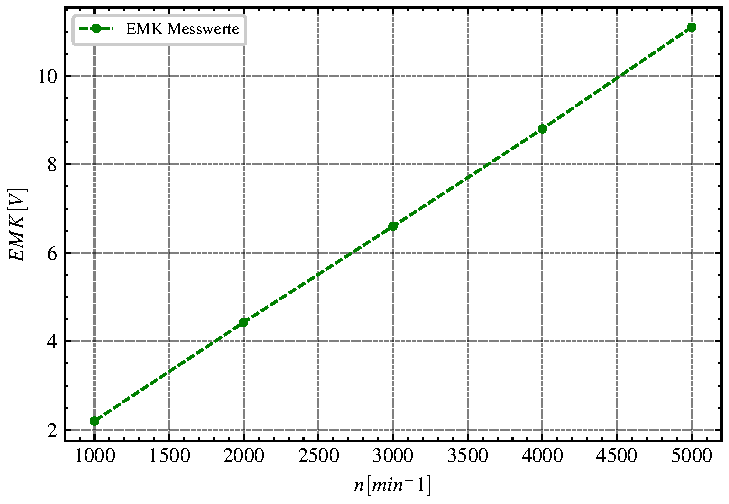
\includegraphics[width=\columnwidth]{plots/4.1_Leerlaufversuch.pdf}
    \caption{Idle Mode}
    \label{fig:Anlaufmoment}
\end{figure}


\section{loaded generator mode}
In the generator mode the generator is powering the machine. The rotations per minute are set at 4000rpm.
In the previouse experiment we meassured the motor voltage at 4000rpm. Through out this experiment this voltage will be kept at $U_A(4000rpm) = 9.61$.
The load resistors are getting conneted into the cicuite one by one.


\begin{figure}[htbp]
    \centering
    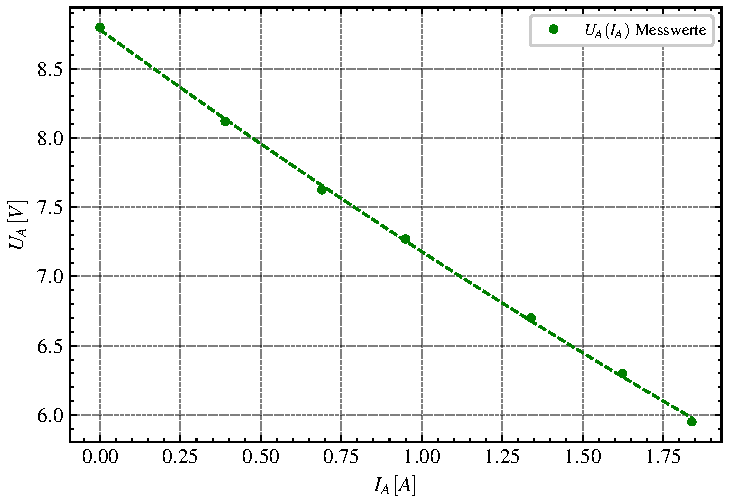
\includegraphics[width=\columnwidth]{plots/4.2_Belasteter_Generator_4000.pdf}
    \caption{loaded generator mode}
    \label{fig:Anlaufmoment}
\end{figure}

To determin the resistance $R_A$ of the generator we need the potential over said resistor as well as the current running through it.\\

\begin{equation}
    R_A = \frac{U_{RA}}{I_A} = \frac{U_A - U_q}{I_A} = ??????
\end{equation}


\section{loaded motor mode}
In the motor mode the voltage $U_A$ is kept konstant, first at 9V later at 12V.


\begin{table}[htbp]
   \centering
   \begin{tabularx}{\columnwidth}{XXXXXXX}
      \toprule
      Switches    & $n [min^{-1}]$ & $I_A [A]$ & Weight$[g]$ & $M[m\, Nm]$ \\
      \midrule
      All Open    & 3766           & 0.386     & 8.08        & 7.924       \\
      S1          & 3548           & 0.724     & 9.29        & 9.110       \\
      S2          & 3385           & 0.958     & 10.75       & 10.54       \\
      S1+S2       & 3261           & 1.146     & 11.53       & 11.31       \\
      S1+S2+S3    & 3080           & 1.400     & 13.75       & 13.48       \\
      S1+S2+S3+S4 & 2962           & 1.565     & 15.15       & 14.86       \\
      All Closed  & 2868           & 1.680     & 16.70       & 16.38       \\
      \bottomrule
   \end{tabularx}
   \caption{Belasteter Motor $U_A=9V$}
\end{table}

\begin{table}[htbp]
   \centering
   \begin{tabularx}{\columnwidth}{XXXXXXX}
      \toprule
      Switches    & $n [min^{-1}]$ & $I_A ,[A]$ & Weight $[g]$ & $M [m\,Nm]$ \\
      \midrule
      All Open    & 5100           & 0.41       & 8.06         & 7.90        \\
      S1          & 4760           & 0.87       & 8.66         & 8.49        \\
      S2          & 4563           & 1.20       & 9.22         & 9.04        \\
      S1+S2       & 4390           & 1.44       & 10.15        & 9.95        \\
      S1+S2+S3    & 4150           & 178.00     & 12.48        & 12.24       \\
      S1+S2+S3+S4 & 3980           & 2.02       & 14.60        & 14.32       \\
      All Closed  & 3910           & 2.20       & 16.93        & 16.60       \\
      \bottomrule
   \end{tabularx}
   \caption{Loaded motor mode - $U_A=12V$}
\end{table}


\begin{figure}[htbp]
    \centering
    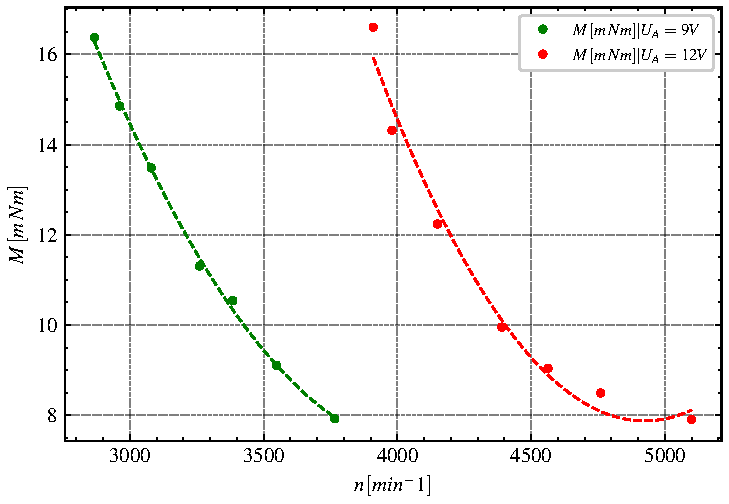
\includegraphics[width=\columnwidth]{plots/4.3_Belasteter_Motor_UA9V_12V.pdf}
    \caption{loaded motor mode}
    \label{fig:Anlaufmoment}
\end{figure}

\end{document}
